\documentclass[12pt]{article}
\usepackage[spanish,es-tabla,es-nodecimaldot]{babel}
\usepackage[round]{natbib}
\usepackage[utf8]{inputenc}

\title{\textbf{Desigualdad económica y su influencia sobre la percepción de las diferencias de ingreso legítimas}}
\author{Julio Iturra Sanhueza \and Catalina Rufs \and Juan Carlos Castillo}
\date{}

\begin{document}
	
\maketitle

\section*{Introducción}

La desigualdad económica es una característica común de gran parte de las sociedades modernas y ha ido en aumento desde la segunda mitad del siglo XX \citep{Esping_Andersen2007}. Aun cuando esta tendencia está siendo impulsada principalmente por el estrato superior de ingresos y sería, por ende, de interés para la mayor parte de la población que haya más redistribución de recursos desde una perspectiva económica de elección racional, la presión social y preocupación pública por esta temática no ha aumentado en conjunto con el alza mencionado \citep{Trump2017}. Este contra-intuitivo escenario es el que explora Kris-Stella \cite{Trump2017} de manera experimental en dos contextos distintos, Estados Unidos -país sumamente desigual a nivel mundial- y Suecia -país con menor nivel de desigualdad-, argumentando a través de la hipótesis de ajuste que la percepción del nivel de desigualdad de ingresos a nivel contextual afectará el nivel de desigualdad que los individuos de esa sociedad consideren legítimo. 

Este argumento fue explorado con antelación por \cite{Castillo2011} en Chile, país que, aun cuando ha presentado una disminución moderada en su desigualdad  durante la última década, sigue estando dentro de los más desiguales del mundo \citep{PNUD2015,WDI2018}. Los resultados de esa investigación van en la línea de los experimentos realizados por \cite{Trump2017}, donde se ha evidenciado que existe una mayor justificación de desigualdad de ingresos cuando se percibe mayores brechas en estos. En relación a la evidencia señalada, este artículo tiene por objetivo profundizar los hallazgos para Chile respecto de cómo afecta la percepción de la desigualdad de ingresos en la legitimación de mayores diferencias entre los ingresos más altos y más bajos, inspirándose en el experimento diseñado por \cite{Trump2017}.

\subsection*{Marco Teórico}


La presencia sostenida de  desigualdad en las sociedades modernas se ha desarrollado en el contexto que los estratos de mayores ingresos, han sido quienes han tenido mayor influencia producto del aumento de sus riquezas \citep{Atkinson2011,Volscho2012}. Ante este escenario, desde una perspectiva de interés-propio \citep{Meltzer1981} se esperaría que la mayor parte de la población estuviera en desacuerdo con la desigualdad existente. Esto, dado que sería beneficioso para ellos que existiera un aumento en la redistribución de recursos que les permitiera acceso a mayores niveles de estos. Entonces, ¿por qué el aumento de la desigualdad no viene acompañado de un incremento sistemático de la disconformidad y consecuente demanda por redistribución? La respuesta que se ha formulado es que esto ocurre dado que la percepción de desigualdad de ingresos existente en un contexto, afecta el nivel de justificación y/o legitimación de la desigualdad entre sus individuos \citep{Trump2017, Castilloetal2019}. Los mecanismos a través de los cuales esto ocurre serán explorados a continuación, en conjunto con precisiones conceptuales relevantes para el estudio. 

En primer lugar, es necesario definir conceptualmente qué significa \textit{justificar} o \textit{legitimar} cierto nivel de desigualdad. Muchas veces estos dos conceptos se han utilizado de manera poco precisa como sinónimos \cite{Castillo2011}, cuando en realidad la justificación individual de un nivel de desigualdad en particular, no implica necesariamente que exista legitimidad de esta. La diferencia yace en que la legitimación de algo (autoridad, desigualdad, justicia, etc.) no proviene de un consentimiento privado, sino que de uno colectivo  \citep{Walker1993}; es decir, requiere de la aceptación de grupos sociales de estatus variados, lo cual implica que exista validez a pesar del beneficio personal asociado a esta \citep{Weber1947}. Esto último es sumamente relevante en la justificación de la desigualdad de ingresos, ya que necesitaría de un consenso entre grupos sociales que fuera por sobre el interés propio al respecto. Entonces, dado que nuestra variable central en estudio es la justificación de la desigualdad operacionalizada desde la diferencia recomendada o "justa" -establecida por un individuo- entre los salarios de dos ocupaciones de estatus extremos , para comprobar legitimidad como propuso \cite{Castillo2011} en su investigación, habrá que evaluar si existen o no diferencias entre grupos de distintos niveles de estatus.


Con esa precisión conceptual establecida, a continuación, se profundizará en los mecanismos que pueden mediar el cómo la percepción de mayor desigualdad de ingresos puede significar una mayor legitimidad de esta en un contexto dado. \cite{Shepelak1986} examinaron el efecto que tenía la realidad en la que vivían las personas en su percepción sobre cómo debería ser esa realidad en torno al tema de justicias distributivas. Esta teoría plantea que las personas responden ante estándares existenciales de justicia, lo cual significa que los estándares de justicia que cada individuo recomiende estarán afectados por los estándares reales -o mejor dicho, percibidos de la realidad- que existan en el contexto en el que se encuentre. En términos simples esto significa que la distribución actual de los recursos en un contexto va a influir en el consenso sobre cuánta desigualdad es justificable \citep{Castilloetal2019}. Esto se produce, en parte, por la hipótesis de ajuste propuesta por \cite{Trump2017} . Ante la pregunta de por qué frente a mayor desigualdad de ingresos no se produce un incremento en la demanda por mayor redistribución, esta hipótesis sugiere que los individuos tienden a justificar la desigualdad a partir de procesos cognitivos, lo que tiene como resultado un aumento de la brecha de ingresos que se considera justa. 

El proceso psicológico de ajuste planteado por la hipótesis, se dar a partir de dos vías: (1) sesgo de status quo y (2) teoría de justificación del sistema \citep{Trump2017}. El sesgo de status quo ocurre cuando las personas adaptan sus expectativas de la realidad - desigualdad legítima en este caso - por justificaciones racionales, y también, por anclaje. El ajuste racional se produce cuando, a partir de datos fácticos del contexto, las personas cambian su opinión respecto de cómo debiesen ser las cosas \citep{Trump2017}. Un ejemplo de ello lo entrega esta misma autora, Kriss-Stella \cite{Trump2017}; supongamos que una persona recibe información respecto de cuánto es el sueldo de un oficio o profesión en particular. A través del ajuste racional, la persona intentará justificar ese monto con razones como el esfuerzo, la inversión o la productividad que implica esa carrera, por ejemplo, y así ajustará sus apreciaciones respecto de cuánto debería ganar.

En conjunto con el sesgo de la racionalidad viene el efecto de anclaje, el cual es una de las heurísticas cognitivas más robustas \citep{Furnham2011}. La heurística, que se caracteriza por permitir a la cognición una respuesta intuitiva y rápida a modo de reducir la complejidad para predecir valores, fue acuñada para proponer un modelo alternativo de comportamiento económico racional, basado en la racionalidad limitada \citep{Simon1955}. Entonces, el efecto de anclaje es la gran influencia que tiene un valor presentado inicialmente en los tomadores de decisiones, la cual sesga su juicio \citep{Tversky1974}. Desde el ámbito de la justicia distributiva, \cite{Markovsky1988} plantea que la opinión sobre una recompensa justa puede estar sesgada por una recompensa ancla de conocimiento previo, si es que esa ancla está en la misma escala que la respuesta sobre la recompensa justa. Por lo tanto, siguiendo el mismo ejemplo utilizado por \cite{Trump2017}, si a una persona se le dice cuánto gana una profesión u oficio en particular, este monto puede funcionar como un ancla que luego sesga la respuesta respecto de cuánto cree que debería o sería justo ganar. 

Si el ejemplo anteriormente utilizado se amplía al concepto de desigualdad, el conocimiento de cuánto es la diferencia salarial entre dos ocupaciones, la de más y la de menos prestigio, producirá sesgos racionales y de anclaje en cuanto a la desigualdad que una persona considera justa o recomienda. \cite{Wegener1987} sostiene que las personas creen que la distribución de recursos o asignación de sueldos actual es justa porque no tienen conocimiento de cómo se distribuyen en realidad. Esto las vuelve propensas a sesgarse por la información de la que disponen, lo que él denomina la ilusión de la justicia distributiva. Es relevante destacar esto, ya que el tipo de información respecto de la realidad distributiva al que accede cada persona estará determinado por su posición en la jerarquía social \citep{Castillo2011}. Por lo tanto, es de esperar que cada grupo social perciba y recomiende distintos niveles de desigualdad. Entonces, para poder evaluar la legitimidad consensuada no se debe esperar que todos recomienden los mismos niveles de desigualdad, pero sí que las diferencias entre cuanto perciben y recomiendan sean proporcionalmente iguales entre los distintos grupos sociales. 

El segundo mecanismo sicológico de ajuste afecta cómo la percepción de mayor desigualdad puede significar una mayor legitimidad de esta en un contexto dado, proviene de la teoría de justificación de sistema \cite{Trump2017}. Melvin Lerner se preguntó cómo es que aquellos sistemas que generan sufrimiento son capaces de mantener el apoyo popular \citep{Lerner1966} .  Esta teoría postula que el ser humano tiende a apoyar y defender el status quo social \citep{Blasi2006}, de modo tal que el sistema en el que vive es considerado justo y legítimo con el objetivo de reducir el malestar y estrés sicológico que  produce la idea contraria. Así, este ajuste tiene como resultado la legitimación de la información que reciben sobre el sistema distributivo \citep{Trump2017}. Desde esta teoría, es plausible sostener que al recibir información respecto a cuan desigual es la distribución de recursos, los individuos tienden a  justificarla y validarla acríticamente ,a modo de sentirse cómodos en el status quo, y luego recomienden como justos niveles superiores de desigualdad. 

Dicho lo anterior, esto no implica que las personas siempre acepten las injusticias. No obstante, frente a  las distintas interpretaciones factibles, los individuos poseen sesgos con respecto a preferir situaciones que generen menores grados de disonancia cognitiva \citep{Trump2017}. Para medir de manera más directa esta última teoría descrita, acudiremos a la escala creada por \cite{Rubin1975}, Creencia en un mundo justo . A a través de ella recabaron evidencia de que muchas personas creen que el mundo es un lugar donde las buenas personas son recompensadas y las malas castigadas, admirando a personas afortunadas y mirando en menos a aquellas que no lo son. Su versión más actual Creencia global en un mundo justo de \cite{Lipkus1991} está correlacionada con la motivación de justificación del sistema, ya que mide la creencia por parte de las personas de que el mundo donde viven es justo. Entonces, mediante esta escala se podrá operacionalizar el sesgo sicológico de justificación de sistemas, el cual debiese producir que aquellos que mayores puntajes alcancen, también validen mayores niveles de desigualdad como justos.   

La variable central de esta investigación es la desigualdad recomendada. En ella se podrá explorar el efecto de cuánta desigualdad percibían anteriormente, para probar la hipótesis de ajuste y también, el efecto que tiene en ello los distintos tratamientos que se realicen, los cuales serán explicados en detalle en la sección siguiente. Además, a través de las variables que se operacionalicen para medir status y grupo social se podrá medir si existen diferencias entre estos en las desigualdades recomendadas -controlando por percepción de desigualdad-, a modo de explorar si la teoría de elección racional juega un papel relevante o bien, el contexto brinda un nivel de desigualdad legítimo. 


\newpage
\section*{Datos, variables y método}

\emph{Midiendo las actitudes hacia las Diferencias de Ingreso Legítimas}

Al que igual \cite{Trump2017}, nuestra variable dependiente es la actitud hacia las diferencias de ingreso. Lo que se busca conocer es la opinión con respecto a qué tan grandes deberían estas diferencias entre ocupaciones de distinto estatus. Para realizar la medición de esta actitud, decidimos emplear las preguntas que ha utilizado previamente en Chile el módulo Social Inequality del \emph{International Social Survey Programme}. Se les pregunta a los encuestados cuánto dinero creen que \emph{gana} una lista de ocupaciones en un año, después se les pregunta cuánto creen que estas ocupaciones \emph{deberían} ganar en un año. Con esto es posible conocer el nivel de desigualdad \emph{percibida} por los individuos, como también conocer el nivel de desigualdad que \emph{recomiendan} o que consideran justa.

Las ocupaciones que se presentaron son ``Un profesor de educación básica'', ``Un ministro de Gobierno chileno'', Un obrero no calificado de una fábrica, Un dueño de una pequeña empresa, ``Un gerente de una gran empresa'' y ``Un doctor o médico de medicina general''. El orden en el que se posicionaron las ocupaciones se realizó de manera aleatoria. La operacionalización de la variable dependiente se realizó a través del Índice de justicia \citep{Jasso1999}. Esta medida permite conocer la desigualdad percibida y recomendada a través la función \emph{(ln({Ocupación alto estatus / Ocupación bajo estatus}))}. Un número más alto, indica una mayor brecha entre el salario de la ocupación de alto estatus con la de estatus bajo. 

Dicho lo anterior, empleamos dos medidas basadas en el índice de justicia. La ecuación \ref{eq1} representa la medida empelada por \cite{Trump2017}, donde no se consideran las ocupaciones específicas, razón por la cual se utiliza el salario máximo y mínimo mencionado por el entrevistado. Esto se debe a que el interés principal es conocer la desigualdad, tanto percibida como recomendada, desde un punto de vista global.

\begin{equation}
\label{eq1}
D_1 = \ln\Bigg(\frac{\text{Máximo salario recomendado}}{\text{Mínimo salario recomendado}} \Bigg)
\end{equation}
%ECUACION1

Adicionalmente, calculamos el mismo índice en base al salario de la ocupación de mayor y menor estatus \citep{Jasso1999}, media que ha sido empleadas anteriormente en estudios realizados en Chile \citep{Castillo2012justice,Castillo2012} y que permite disponer de una aproximación adicional a la desigualdad percibida y al salario justo. Para el cálculo del índice, la ecuación \ref{eq2} muestra que el salario de ``Un gerente de una gran empresa'' es la ocupación de mayor estatus y que el salario de ``Un obrero no calificado de una fábrica'' es la ocupación de menor estatus.

%ECUACION2

\begin{equation}
\begin{aligned}
\label{eq2}
D_2  = \ln\Bigg(\frac{\text{Salario Gerente}}{\text{Salario Obrero}}\Bigg)
\end{aligned}
\end{equation}
	
\subsection*{Experimento}\label{experimento}

Entre noviembre y diciembre de 2014 se realizó una encuesta de corte transversal titulada ``Creencias políticas y sociales''. El estudio se realizó en individuos adultos con edad entre 18 y 87 años de sectores urbanos de la Región Metropolitana. El método de administración del cuestionario fue de manera presencial y asistido por \emph{Tablet}. La media de edad de los participantes es de 44 años, 62\% son mujeres, 18\% tiene educación terciaria o superior y un 54\% declara no tener posición política.

Una parte de la muestra (226 participantes) corresponde al grupo control: estos no recibieron tratamiento de información, respondieron preguntas sociodemográficas, la escala de Creencia en un Mundo Justo (CMJ),\footnote{En base a los criterios señalados por \cite{Brown2008}, se realizó un Análisis Factorial Confirmatorio que evidenció un buen ajuste de la escala para la Creencia en un Mundo Justo (\(\chi^2(5)\)=8.40, \(p\)=0.015, CFI=0.99, RMSEA=0.06). En base a esta evidencia, se procedió a crear un índice promedio con los ítems.} seguido de las preguntas sobre desigualdad salarial percibida y justa. Adicionalmente, se emplearon 2 tratamientos en tres combinaciones distintas. Posteriormente a responder a la pregunta sobre cuánto \emph{cree que gana} mensualmente cada una de las seis ocupaciones, el primer grupo (\emph{n}=104) recibió información sobre las consecuencias de la reforma educacional en producir mayor equidad, además una lista de salarios para las seis ocupaciones mencionadas en la pregunta cuánto gana cada ocupación. El segundo grupo (\emph{n}=148) solo recibió la información del párrafo; y finalmente, al tercer grupo (\emph{n}=254) solo se les mostró la información de la lista de salarios. Luego de recibir esta información, se le preguntó a los encuestados cuánto \emph{cree que deberían ganar} mensualmente cada una de las seis ocupaciones. En la Información Sumplementaria se provee de una tabla de balance de la asignación aleatoria.

El sección siguiente se presentarán los resultados del análisis. Se estimaron una serie de modelos de regresión para determinar si la exposición a información sobre desigualdad tiene un efecto sobre la desigualdad recomendada. Con el objetivo de poner a prueba la robustez de los resultados, se incluyeron como controles la escala de Creencia en un Mundo Justo (CMJ), posición política, nivel educacional y Desigualdad percibida.  

%\begin{figure}[H]
%	\centering 
%	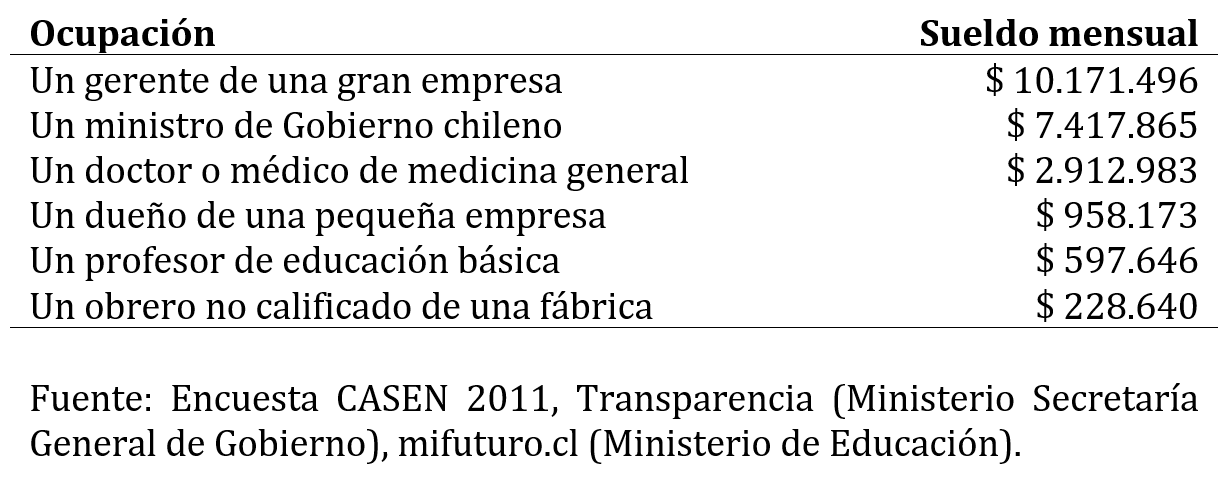
\includegraphics[width=10cm]{Resultados/images/treat1} 
%	\caption{Lista de salarios por ocupación}
%	\label{treat1}
%\end{figure}

\begin{table}[H]
\begin{center}
\caption{Lista de salarios por ocupación}
\begin{tabular}{ll}
\toprule
\textbf{Ocupación}                                                                            										 &\textbf{Sueldo mensual} \\ 
\midrule
Un gerente de una gran empresa                                                                                                 & \$ 10.171.496           \\
Un ministro de Gobierno chileno                                                                                                & \$ 7.417.865            \\
Un doctor o médico de medicina general                                                                                         & \$ 2.912.983            \\
Un dueño de una pequeña empresa                                                                                                & \$  958.173             \\
Un profesor de educación básica                                                                                                & \$  597.646             \\
Un obrero no calificado de una fábrica                                                                                         & \$  228.640             \\
\bottomrule																													  
%\multicolumn{2}{m{\textwidth}}{\footnotesize \textit{\textbf{Fuente}}: Encuesta CASEN 2011, Transparencia (Ministerio Secretaría General de Gobierno), mifuturo.cl (Ministerio de Educación).}
\multicolumn{2}{m{11cm}}{\footnotesize{\parbox{1.0\linewidth}{\vspace{2pt} \textbf{\textit{Fuente}}: Encuesta CASEN 2011, Transparencia (Ministerio Secretaría General de Gobierno). www.mifuturo.cl (Ministerio de Educación).}}} 
\end{tabular}
\end{center}
\end{table}

\newpage
\section*{Resultados y discusión}



En primer lugar, es relevante destacar que un 82\% de los participantes percibe que la brecha entre el salario de las ocupaciones de mayor y de menor estatus es menor a la que realmente es según los datos CASEN 2011. Esta información nos hace estar seguros de que, al aplicar los tratamientos, efectivamente estamos ajustando su percepción de desigualdad hacia arriba al informarles de que existe más de la que ellos pensaban. 

Los resultados generales del experimento son presentados en la Figura 1 para la desigualdad recomendada en base al máximo y mínimo salario mencionado. Así también, los resultados para la desigualdad recomendada en base al salario de las ocupaciones de alto y bajo esta tus son presentados en la Figura \ref{fig:barplot2} y la Tabla \ref{tab:logcov}. A partir de la Figura 1, se tiene que luego de recibir el tratamiento de información sobre desigualdad, es posible evidenciar que no existe una diferencia significativa en términos de la desigualdad recomendada -en base al máximo y mínimo salario mencionado- para cada una de las condiciones. Estos resultados sugieren que, contrario a lo que se esperaba, mayor información respecto a la desigualdad no impacta en cuánta desigualdad se prefiere en términos globales.
   

%TABLA CON DESCRIPTIVOS DE LAS DEPENDIENTES

\begin{figure}[H]	
\centering 
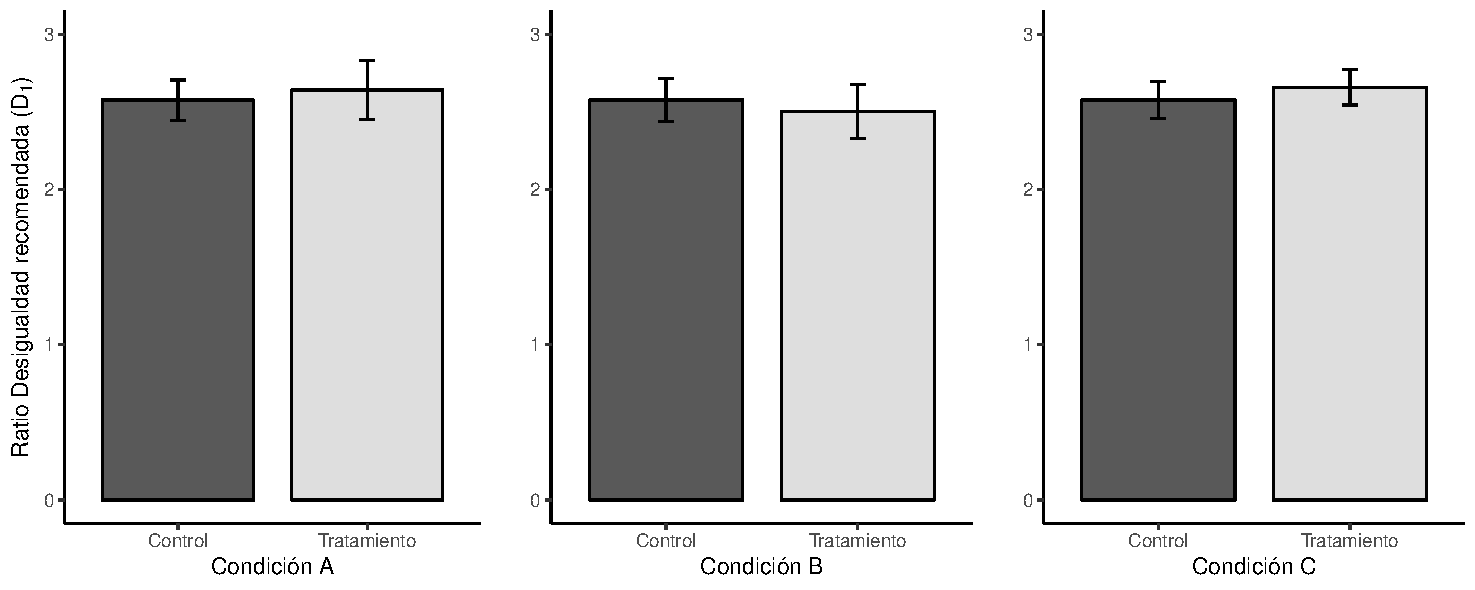
\includegraphics[width=0.85\linewidth]{Resultados/images/barplot1} 
\caption{Resultados del experimento, en base a los valores predichos para la desigualdad recomendada general}
\label{fig:barplot1}
\end{figure}


Conforme a lo anterior, se realizó el análisis para determinar el efecto del tratamiento sobre la desigualdad recomendada en base al índice propuesto por \cite{Jasso1999}, considerando el salario recomendado para las ocupaciones de alto y bajo estatus. Se evidenció que luego de recibir el tratamiento de información de la condición A -lista de salarios reales y párrafo sobre consecuencias de la reforma educacional-, la desigualdad recomendada incrementó en 0,55. Esto ya que el grupo tratado recomienda 2,32 en contraste con 1.77 del grupo control (p<0.001), lo cual representa un cambio aproximado de un 31\%. Por otro lado, se evidenció que el tratamiento de información de la condición B, basado en el párrafo sobre la reforma educacional, no afecta el nivel de desigualdad que prefieren los individuos. Si bien existe un incremento de 0,23 en la desigualdad recomendada, el tratamiento no produce una diferencia estadísticamente significativa respecto al grupo control. Finalmente, se evidenció que obtener información sobre la desigualdad salarial según ocupación -tratamiento de información bajo la condición C-, produce un cambio de 0,32 en la desigualdad recomendada, equivalente a un incremento de 18\% respecto al grupo control. En ambos tratamientos significativos, el alza se dio porque las personas tendieron a recomendar mayor salario para el gerente y dejar igual a los obreros (Ver en Anexos Figura \ref{fig:obgapb} y \ref{fig:gergapb}). 

Lo anterior confirma la hipótesis respecto de que, al modificar la percepción de desigualdad de las personas mediante información sobre las altas diferencias entre los salarios distintas ocupaciones, ellas tienden a recomendar mayores niveles de desigualdad. Esto podría estar ocurriendo por la hipótesis de ajuste discutida en el marco teórico  \citep{Trump2017}, a partir del sesgo de ancla y de la justificación racional. Es interesante el que el ajuste cognitivo ocurra a partir de ver las cifras y no al ver el párrafo que induce percepción de mayor desigualdad. Esto da luces respecto de que efectivamente el mecanismo a través del cual se produce el ajuste puede ser el sesgo de anclaje, dado que la persona se ancla a la cifra que ya vio, y/o el ajuste racional, en el que la persona justifica racionalmente por qué tal ocupación gana lo que gana y por ende, luego recomienda más desigualdad. Estos resultados no dan luces de la teoría de justificación de sistemas, particularmente porque desde esta se esperaría que el párrafo que inducía percepción de desigualdad hubiese producido un ajuste significativo en la recomendación de desigualdad, por el esfuerzo de las personas de validar el sistema injusto en el que viven. 

\begin{figure}[H]
	\centering 
	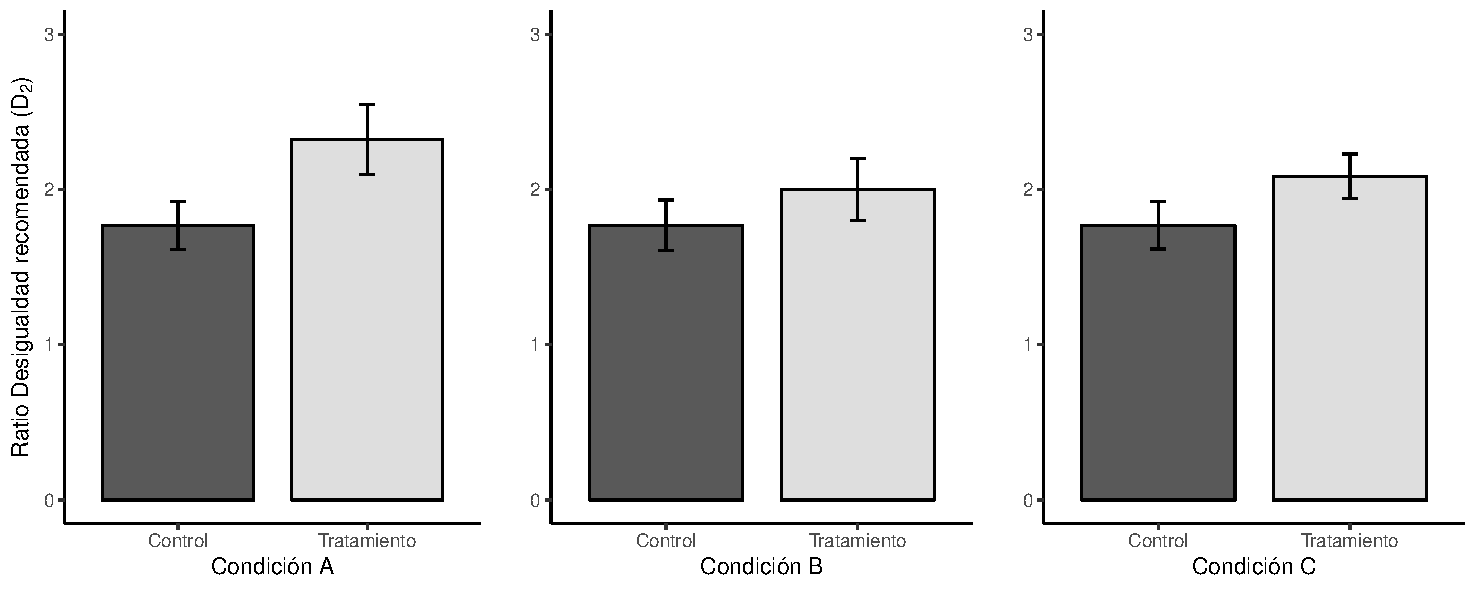
\includegraphics[width=0.85\linewidth]{Resultados/images/barplot2} 
	\caption{Resultados del experimento, en base a los valores predichos para la desigualdad recomendada según ocupaciones de alto y bajo estatus}
	\label{fig:barplot2}
\end{figure}


\renewcommand{\arraystretch}{1}
\renewcommand{\baselinestretch}{1}

\begin{table}[H]
\caption{Modelos de regresión para desigualdad recomendada}
\begin{center}
\scalebox{0.75}{
\begin{tabular}{l@{} D{.}{.}{3.5}@{} D{.}{.}{3.5}@{} D{.}{.}{3.5}@{} D{.}{.}{3.5}@{} D{.}{.}{3.5}@{} D{.}{.}{3.5}@{} }
\toprule
& \multicolumn{2}{c}{Condición A}  & \multicolumn{2}{c}{Condición B}  & \multicolumn{2}{c}{Condición C}\\
\cmidrule(l{1pt}r{2pt}){2-3} \cmidrule(l{2pt}r{2pt}){4-5} \cmidrule(l{2pt}r{2pt}){6-7}
& \multicolumn{1}{c}{Modelo 1} & \multicolumn{1}{c}{Modelo 2} & \multicolumn{1}{c}{Modelo 3} & \multicolumn{1}{c}{Modelo 4} & \multicolumn{1}{c}{Modelo 5} & \multicolumn{1}{c}{Modelo 6} \\
\midrule
Tratamiento                 & 0.55^{***} & 0.56^{***} & 0.23       & 0.24       & 0.32^{**}  & 0.30^{**}  \\
                            & (0.14)     & (0.14)     & (0.13)     & (0.14)     & (0.11)     & (0.11)     \\
Creencia Mundo Justo        &            & -0.03      &            & -0.05      &            & -0.04      \\
                            &            & (0.06)     &            & (0.06)     &            & (0.04)     \\
Centro                      &            & 0.36       &            & 0.25       &            & 0.39       \\
                            &            & (0.24)     &            & (0.24)     &            & (0.21)     \\
Derecha                     &            & 0.52^{*}   &            & 0.05       &            & 0.20       \\
                            &            & (0.25)     &            & (0.25)     &            & (0.20)     \\
Ninguno                     &            & -0.05      &            & -0.16      &            & 0.07       \\
                            &            & (0.17)     &            & (0.17)     &            & (0.14)     \\
No sabe                     &            & 0.64       &            & 0.36       &            & 0.38       \\
                            &            & (0.43)     &            & (0.43)     &            & (0.37)     \\
Desigualdad percibida (Log) &            & 0.16^{**}  &            & 0.12^{*}   &            & 0.10^{*}   \\
                            &            & (0.06)     &            & (0.06)     &            & (0.05)     \\
Educación                   &            & 0.03       &            & 0.04       &            & 0.06^{*}   \\
                            &            & (0.03)     &            & (0.03)     &            & (0.03)     \\
Intercepto                  & 1.77^{***} & 1.19^{***} & 1.77^{***} & 1.39^{***} & 1.77^{***} & 1.18^{***} \\
                            & (0.08)     & (0.33)     & (0.08)     & (0.33)     & (0.08)     & (0.27)     \\
\midrule
Adj. R$^2$                  & 0.04       & 0.09       & 0.01       & 0.03       & 0.02       & 0.04       \\
%Num. obs.                   & 325        & 311        & 366        & 340        & 471        & 446        \\
\textit{N}   & \multicolumn{1}{c}{325} & \multicolumn{1}{c}{311} & \multicolumn{1}{c}{366} & \multicolumn{1}{c}{340} & \multicolumn{1}{c}{471} & \multicolumn{1}{c}{446} \\
\bottomrule
\multicolumn{7}{m{17cm}}{\footnotesize{\parbox{1.0\linewidth}{\vspace{2pt} Errores estándar robustos entre paréntesis.  \\ 
			$^{***}p<0.001$, $^{**}p<0.01$, $^*p<0.05$. \\
			\textbf{\textit{Nota}}: Condición A, corresponde al tratamiento con el párrafo sobre la reforma educacional y la lista de salarios. Condición B, es el párrafo unicamente; y Condición C es la lista de salarios por ocupación.}}} 
\end{tabular}
}
\label{tab:logcov}
\end{center}
\end{table}



La Tabla \ref{tab:logcov} muestra que el efecto de la exposición a la condición de desigualdad se mantiene cuando se controla por la creencia en un mundo justo, la posición política, percepción de desigualdad y educación. Estos resultados ofrecen evidencia a favor de la hipótesis de ajuste, de modo tal que el grado de información respecto a la desigualdad tiene como consecuencia una mayor desigualdad recomendada en términos de la brecha salarial entre ocupaciones de alto y bajo estatus, aun cuando se controle por otras variables relevantes. 

Es llamativo que la creencia en un mundo justo no presente una asociación estadísticamente significativa si se considera su alta correlación con la hipótesis de justificación de sistemas. Esto quiere decir que creer más en un mundo justo, implica un mayor nivel de justificación del sistema y por tanto, era de esperar que tuviera una relación positiva con recomendar mayores niveles de desigualdad. En la Tabla \ref{tab:logcov} se observa que esta hipótesis no se cumple ni en dirección, ya que presenta coeficientes negativos en dos de los tratamientos, ni en magnitud, dado que en la tercera condición tiene valor cero y no es estadísticamente significativa en ningún modelo. Este resultado va en línea con lo antes mencionado respecto del efecto no significativo del tratamiento del párrafo y difiere de lo obtenido por \cite{Trump2017} para el contexto estadounidense y Sueco, donde sí se cumple la hipótesis. Por esto, sería interesante analizar en futuras investigaciones qué ocurre particularmente en la sociedad chilena con la teoría de justificación de sistemas. \cite{Trump2017} propone un diseño experimental para estudiarlo. 
  
Respecto del coeficiente positivo y estadísticamente significativo de percepción de desigualdad, cumple con las expectativas del estudio sobre que a mayores percepciones de desigualdad, las personas tienden a justificar una mayor brecha salarial debido a procesos de ajuste cognitivo. Por otro lado, desde un enfoque de interés racional, se esperaría que aquellas personas que perciban más ingresos recomienden mayores niveles de desigualdad debido a que es beneficioso para ellos. En la Tabla \ref{tab:logcov} podemos ver que la variable educación -la cual fue utilizada como un proxy de nivel socioeconómico-, aparece como positiva y significativa en el Modelo 3. Es decir, tener mayores niveles de educación se asocia con recomendar mayores niveles de desigualdad. 

Esto último va en consonancia con un enfoque de interés racional \citep{Meltzer1981}, lo cual da cuenta de que individuos de mayor estatus tienden a justificar mayor desigualdad. Así también, es relevante observar que una mayor percepción de desigualdad se asocia con una mayor brecha salarial recomendada. Esta evidencia permite sostener que la justificación de brecha salariales se explica, por un lado, por el estatus social de los individuos, así como también por los niveles de desigualdad percibida, lo cual va en consonancia con los hallazgos reportados por \cite{Trump2017} para el contexto estadounidense y sueco.

\section*{Conclusiones}
 
El presente trabajo ha evidenciado que la desigualdad recomendada se ve afectada por la percepción de desigualdad, específicamente cuando los individuos son consientes de la brecha salarial real. En base a la hipótesis propuesta, se ha evidenciado que tener mayor información con respecto a la desigualdad económica tiene como consecuencia que los individuos recomienden una mayor brecha salarial entre ocupaciones de bajo y alto estatus. En este sentido, se emplearon dos tratamientos en tres combinaciones distintas, donde la información  respecto a los salarios afecta sustantivamente la magnitud de desigualdad recomendada, mientras que obtener información con respecto a las consecuencias de largo plazo que tendría la reforma educacional no afecta significativamente la brecha salarial recomendada. Así también, se evidenció que la combinación de ambos tratamientos posee un efecto promedio más alto que cada condición de manera individual. 

En un principio, se postuló la interrogante con respecto a si la hipótesis de ajuste cognitivo de expectativas se cumpliría para el contexto de Chile. \cite{Trump2017} evidenció que en contextos con diversos grados desigualdad económica y diferencias sustantivas en términos de políticas de bienestar, poseer mayor información con respecto a la desigualdad económica sí afecta la desigualdad que recomiendan los individuos. En nuestro estudio empleamos dos medidas diferentes para abordar el análisis de la desigualdad recomendada, por un lado empleamos la medida que utilizó Trump para analizar la desigualdad general, donde no se evidenciaron diferencias significativas ente los distintos grupos de estudio. Por otro lado, decidimos emplear la medida propuesta por \cite{Jasso1999} como alternativa a lo realizado por Trump, evidenciando que la información sobre desigualdad salarial tiene un efecto sustantivo en la desigualdad recomendada según ocupaciones de alto y bajo estatus.

En base a esta evidencia, es factible sostener que las percepciones relacionadas con la desigualdad, y en particular con la desigualdad salarial, posee consecuencias sustantivas en cómo los individuos racionalizan estas diferencias. Desde la literatura sobre preferencias redistributivas, se sostiene que contextos más desiguales se asocian con mayor demanda por redistribución. No obstante, aquí sostenemos que el efecto de la información es robusto sobre la brecha salarial recomendada, independiente de la posición política, estatus social y creencias distributivas. 

Dicho lo anterior, nuestros resultados tiene implicancias en el estudio de las preferencias redistributivas en contextos de alta desigualdad y con diversas políticas de bienestar social, tal como ocurre en los distintos países de América Latina. Así,  se abre la interrogante con respecto a cómo se asocia la desigualdad recomendada con la redistribución, o sobre qué ámbitos de política social se encuentra relacionado. Se ha evidenciado que el apoyo a distintas medidas redistributivas varía según el tópico en evaluación teniendo presente que la \textit{necesidad} es distinta al ser \textit{merecedor} \citep{Jensen2017,Aaroe2014}. Esta racionalidad opera como diferenciador en el apoyo a políticas sociales en salud o pensiones de vejez, donde la magnitud de la desigualdad  prefiere es un antecedente relevante cuando se evalúa la asignación de recursos.        
 
A diferencia de los experimentos en contextos cerrados y controlados, la realización de experimentos a través de encuestas ofrece la posibilidad de acceder a muestras de mayor tamaño y representatividad. Sin embargo, los resultados del presente estudio deben ser interpretados con cautela debido a que la muestra responde una parte del área urbana de la Región Metropolitana, lo cual imposibilita extrapolar los resultados a la sociedad en su conjunto. Por otro lado, se requiere mayor investigación en términos de que no es posible evidenciar la sostenibilidad temporal del efecto del tratamiento, debido a que las actitudes no son estáticas, en particular aquellas que se relacionan con temas distributivos. Futuras investigaciones deben avanzar hacia un estudio con tamaños muestrales que permitan realizar inferencias a nivel poblacional. En esta línea, recientes avances en el ámbito de la investigación realizada a través de encuestas a través de internet sugieren que la la realización experimentos usando esta estrategia de muestreo tiene la ventaja de ser altamente eficiente en el uso de recursos, además de que permite obtener muestras con niveles de heterogeneidad socioedemográfica y socioeconómica similares a encuestas tradicionales \citep{Zhang2018}.   
  
%-----------------
 
%-- Al decirle a las personas el nivel de desigualdad, tendieron a recomendar más Esto puede estar respondiendo a la hipótesis de ajuste, ya que al cambiar la percepción de las personas sobre la desigualdad ajustan entonces cuánta debiese existir. Podría ser en gran parte por el efecto ancla discutido en el marco teórico ya que el mayor efecto está cuando se muestran las cifras, no así el párrafo. Al ser un experimento, se destaca que esta relación es causal, con la direccionalidad esperada. Con el tratamiento de información, las personas ajustan sus percepciones y por tanto, ajustan sus recomendaciones. 

%-- Podemos ver que en este contexto, aquellos que creen en un mundo justo no presentan cambios en los niveles de recomendación de desigualdad. Dado que esta escala se correlaciona con la hipótesis de justificación de sistema, es interesante analizar en futuras investigaciones qué ocurre particularmente en la sociedad chilena que no hace efecto.

%-- Al igual que en el experimento de K.S. Trump, podemos ver que ser de derecha hace que se recomiende en promedio mayor desigualdad. **habría que ver si "creencia en un mundo justo" tiene una alta correlación con esta de alguna forma. 

%-- Aquellas personas que entraron al experimento percibiendo mayores niveles de desigualdad, como se esperaba, recomiendan mayores niveles de esta también. 

%-- Acordamos de ver el tema de cómo afecta el status-nivel ses, para probar la hipótesis de racionalidad y beneficio propio.  

%-- Aún así, no sabemos si quienes aumentaron sus recomendaciones de desigualdad a la vez aumentaron sus demandas por redistribución. Quizás efectivamente viene acompañado de un aumento de la insatisfacción. Es una limitante de este experimento. Por el marco teórico, habríamos de esperar que no ya que debiesen estar cambiando el parámetro de lo que consideran justo dado los procesos de ajuste. 

% :( en nuestra encuesta no preguntamos al final por satisfacción o insatisfacción de políticas. Pero podemos decir que Trump sí lo justifica, y se espera que no pase acá tampoco.

\newpage 
\def\bibfont{\small}
\bibliography{zlibrary}
\bibliographystyle{apalike}
\appendix


\end{document}

